% analyze five different legal rules
% two steps: social planner's problem, platform behavior under different legal rules
This section is organized as follows: three subsections correspond to three primitive environments (complete info+no externality, complete info+positive externality, incomplete info+positive externality). For each environment, we analyzed five legal rules: (a) immunity, (b) strict liability, (c) free speech law, (d) safe harbor, (e) liability upon notice.

\begin{table}[]
    \centering
\begin{tabular}{c|c}
    $\lambda(x)$ & probability that item $x$ is harmful \\
    $h(x)$ & harm of item $x$ \\
    $P$ & per-item revenue \\ % demand
    $\delta$ & per-item externality \\
    $c$ & per-item investigation cost \\
    $F$ & fixed cost \\
    $s$ & safe harbor threshold
\end{tabular}
\caption{List of mathematical notations for the model}
% inspect/investigate/screen/filter
\end{table}


\subsection{Perfect Information and No Externality}

A platform hosts a continuum of user-generated content, with each item indexed by $x\in[0,1]$. 
Items are heterogeneous in the harm they cause. Let the harms be represented by the function $h(x)$. Without loss of generality, we assume $h(x)$ is a weakly increasing function such that the content is ordered by the ascending harm. We also assume that there is no-harm content ($h(0)=0$).

The inverse demand curve for the content is $Px$, interpreted as the marginal benefit from consuming the $x$-th unit of the content. We assume the demand curve is perfectly elastic such that the marginal consumer benefit is constant at $P$.
There is a fixed cost $F$ of starting up the platform, regardless of how many items of content it hosts.

Content removal decision is modeled as a threshold $\hat{x}\in[0,1]$ such that items $x>\hat{x}$ are removed and items $x\ls\hat{x}$ remains on the platform. 
\footnote{Choosing a threshold is without loss of generality. One can show that removing any subset of the content $\mathcal{X}\subset[0,1]$ is a weakly dominated strategy.}
Given $\hat{x}$, $\int_0^{\hat{x}}h(x)dx$ is the total harm given the amount of content $\hat{x}$, and $P\hat{x}$ is the consumer welfare.
The social welfare function is given by 
\begin{equation}\label{eqn:efficiency_1}
    \max\{\max_{\hat{x}}P\hat{x} - \int_0^{\hat{x}}h(x)dx-F, 0\}.
\end{equation}
Suppose the platform does not shut down, 
the efficient moderation decision $x^e$ is such that
\begin{equation}\label{eqn:efficiency_1_soln}
    h(x^e)=P,
\end{equation}
where $P$ is the marginal cost of removing the marginal item $x^e$, and $h(x^e)$ is the marginal social benefit of removing $x^e$. 
If the fixed cost $F$ is larger enough such that $Px^e - \int_0^{x^e}h(x)dx < F$, social efficiency requires the platform to shut down and carry no content. If instead $Px^e - \int_0^{x^e}h(x)dx \gs F$, social efficiency requires the platform to operate but only carries content $[0,x^e]$.

The goal of the law is to maximize social welfare from the content carried on the platform. The law cannot directly control which items are carried and which are removed. Instead, it can impose a liability $d(x)\ge 0$ for $x\in[0,\hat{x}]$ on the platform for each item of harmful content the platform carries. The law's optimization problem is to choose a value of $d(x)$ that will induce the platform to maximize social welfare.

\textbf{Intermediary immunity} $d(x)=0$.
The platform is profit-maximizing. Since the prevailing market price is $P$, the revenue is $P\hat{x}$, the profit function is given by 
\begin{equation}\label{eqn:profit_ii}
    \max\{\max_{\hat{x}}P\hat{x}-F,0\}.
\end{equation}
Suppose $P<F$, the platform shuts down. Suppose $P\gs F$, the profit-maximizing choice is $x^{\ast}=1$ such that the platform keeps all of the content. Without the threat of liability, the platform has no incentive to remove any of the harmful content. 

\textbf{Strict liability} $d(x)=h(x)$.
Under strict liability, the platform always pays damages $d$ due to the harm caused by the content it hosts. 
The platform's profit maximization problem then becomes
\begin{equation}\label{eqn:profit_sl}
    \max\{\max_{\hat{x}}P\hat{x} - \int_0^{\hat{x}}d(x)dx-F, 0\}.
\end{equation}
Comparing the objective function \eqref{eqn:efficiency_1} with the profit function \eqref{eqn:profit_sl}, we have that the platform's moderation decision $x^{\ast}$ is efficient if $d(x)=h(x)$. 
That is, the optimal level of damages paid by the platform is equal to the harm.
If so, strict liability rule on the platform leads to social optimum. 

Other parameters may determine whether it is socially efficient to remove none, part, or all of the content. But no matter what that efficient outcome is, strict liability will perfectly align the incentive of the platform with that of a social planner.

The following three rules combine both features of strict liability and immunity, and they are popular proposals in the legal debate.

\textbf{Free speech law}.
Free speech law typically follows the negligence strategy of defining an objective standard of care that a reasonable person is expected to follow when acting. One who acts according to that standard of care faces no liability, even if others are harmed. But one who fails to meet that standard is held liable for the resulting harms. In our model, this approach corresponds to defining a threshold of liability as a reasonable person standard and treating different content differently based on the harm:
% must carry ? Must remove rule
\begin{equation}
d(x)=
\lt\{\begin{array}{ll}
    h(x) & \mbox{if $\hat{x}>x^e$ and $x\in[x^e,\hat{x}]$}, \\ % all x or part of x
    0 & \mbox{otherwise}.
\end{array}\rt.
\end{equation}

The platform's profit function under this rule becomes
\begin{equation}\label{eqn:profit_fs}
    \max\{\max_{\hat{x}}P\hat{x} - \int_{x^e}^{\max\{\hat{x},x^e\}}h(x)dx-F, 0\}.
\end{equation}
It follows that the platform's optimal choice is $\hat{x}=x^e$. The free speech law leads to the efficient outcome.


\textbf{Safe harbor provision}.
Safe harbor provision is modeled as a threshold on the total harm. 
\begin{equation}
d(x)=
\lt\{\begin{array}{ll}
    h(x) & \mbox{if $\int_0^{\hat{x}}h(x)dx>s$}, \\
    0 & \mbox{otherwise}.
\end{array}\rt.
\end{equation}
% Q. loss of safe harbor means all the content is liable for $d$, or only part of the content liable for $d$.
If the total harm on the platform exceeds the threshold $s$, the platform loses its safe harbor status and will be held strictly liable for all the hosted content. Otherwise, the platform will be immune from any liability. Suppose the platform loses the safe harbor status, the revenue loss is $\int_0^{\hat{x}}h(x)dx$ whereas the benefit is $P(\hat{x}-x^e)$. Notice that $P(\hat{x}-x^e)<\int_{x^e}^{\hat{x}}h(x)dx<\int_0^{\hat{x}}h(x)dx$, the deviation is definitely not profitable. 
% Napster case: 94% is not enough

Alternatively, the safe harbor provision can be thought of as a policy constraint on the platform's optimization problem. 
\begin{eqnarray}\label{eqn:profit_sh}
\max &&
\hspace{-1em} \{\max_{\hat{x}}P\hat{x}-F,0\}\nn\\
\mbox{s.t.} &&\hspace{-1em} \int_0^{\hat{x}}h(x)dx\ls s %\nn
\end{eqnarray}
The safe harbor constraint is binding if and only if $s<\int_0^1 h(x)dx$. In that case, the optimal removal decision is defined by the equality of the constraint. It follows that if the threshold is properly chosen such that $s=\int_0^{x^e}h(x)dx$, safe harbor provision also leads to the social optimum. 


\textbf{Liability Upon Notice}.
For each item, a unit cost $c$ is required to submit a notice to the platform. Upon receiving a notice on item $x$, the platform faces no liability $d(x)=0$ if the platform takes it down. Otherwise, the platform will be held strictly liable $d(x)=h(x)$ if the platform does not act upon the notice. In this sense, the liability upon notice regime shifts the burden of proof to users. 

The motivation of the users to send a notice is to avoid further harm. Therefore, the users will send a notice if and only if the harm exceeds the cost $h(x)\gs c$. For item $x=h^{-1}(c)$ (where $h^{-1}(\cdot)$ is the inverse function of $H(\cdot)$), users will be indifferent between sending a notice or not. The range of content that expects to receive notice is $[h^{-1}(c),1]$.
Thus under the liability upon notice regime, the platform will be held liable for the content $x\in [0,\hat{x}]\cap[h^{-1}(c),1]$.  

The platform's profit function becomes
\begin{equation}\label{eqn:profit_lun}
    \max\{\max_{\hat{x}}P\hat{x} - \int_{h^{-1}(c)}^{\max\{\hat{x},h^{-1}(c)\}}h(x)dx-F, 0\}.
\end{equation}
If $\hat{x}<h^{-1}(c)$, the platform will not be held liable for any content it hosts and the marginal revenue of hosting an additional item is $P$, so the profit-maximizing $\hat{x}$ is at least $h^{-1}(c)$. The net marginal benefit changes to $P-h(x)$ once $\hat{x}\gs h^{-1}(c)$. Now the platform still enjoys the marginal revenue $P$ but has to pay the damage $h(x)$ for the marginal content $x$. As $h(x)$ is weakly increasing, the minimum damage will be $h(h^{-1}(c))=c$. 
If $P>c$, then carrying content beyond $h^{-1}(c)$ is profitable and the optimal choice is $h(\hat{x})=P$ such that $\hat{x}=x^e$. 
If instead $P\ls c$, then the optimal choice is to remove content exactly at the notice cutoff to avoid any liability $\hat{x}=h^{-1}(c)$. 
To sum up, the platform's optimal choice is as follows:
\begin{equation}
\hat{x}=
\lt\{\begin{array}{ll}
    x^e & \mbox{if $P>c$}, \\
    h^{-1}(c) & \mbox{otherwise}.
\end{array}\rt.
\end{equation}
Liability upon notice may lead to social efficiency if the notice cost is less than the marginal revenue. When the notice cost is large, this legal rule is inefficient.

\begin{proposition}
Given perfect information and no externality, strict liability, free speech law, safe harbor provision, and liability upon notice all lead to the efficient moderation outcome.
\end{proposition}

\subsection{Perfect Information and Positive externality}

Content, unlike a product, is non-rival in consumption and non-excludable in use. The public good nature of the content is taken in account in this subsection. 
We model this positive externality of the content as an additional value of each item not captured by the consumer demand. The positive externalities could be the knowledge spillover, the democratic value of the institution, etc.
Denote $\delta$ as the per-item social value.

The social welfare function becomes 
\begin{equation}\label{eqn:efficiency_2}
    \max\{\max_{\hat{x}}P\hat{x} +\delta\hat{x} - \int_0^{\hat{x}}h(x)dx-F, 0\}.
\end{equation}
Suppose the platform does not shut down, the efficient moderation decision $x^e$ is such that 
\begin{equation}\label{eqn:efficiency_2_soln}
    h(x^e)=P+\delta \mbox{ or } x^e=1
\end{equation}
The marginal social cost of removing an item is $P+\delta$ larger than $P$ because of the externality. This leads the social planner to carry more content. If the marginal social cost exceeds the harm of the most harmful content $\Bar{h}:=\max_{x\in\{0,1\}} h(x)$, the efficient solution is to not remove any of the content.

\textbf{Intermediary immunity} $d(x)=0$.
The platform cannot monetize the social benefit of content, thus its moderation will not take that into account. The profit function will be the same as \eqref{eqn:profit_ii}. The profit-maximizing decision is again to keep all the content $x^*=1$. But because of the positive externality, this decision coincides with the socially optimal one if $\delta\gs \Bar{h}-P$. 
\begin{proposition}
If $\delta\gs \Bar{h}-P$, intermediary immunity leads to the efficient moderation outcome.    
\end{proposition}


\textbf{Strict liability} $d(x)=h(x)$.
Profit function is the same as \eqref{eqn:profit_sl}. The profit-maximizing moderation satisfies $h(x^*)=P$. Compared with the efficient moderation, we have $h(x^*)<h(x^e)$ such that $x^*<x^e$ the platform hosts less content than the social planner. Strict liability leads the platform to over-remove content than what would be socially desirable otherwise. This happens because the platform does not internalize the social value of content.

\textbf{Free speech law}.
The reasonable person standard will take into account the positive externality such that the threshold of liability will be higher than the no externality case. The profit function is the same as \eqref{eqn:profit_fs}. For item $x\in[0,x^e]$, carrying them imposes no liability and generates marginal revenue $P$, so the platform will choose $\hat{x}$ at least as large as $x^e$. For item $x\in[x^e,1]$, the liability is at least $h(x^e)=P+\delta>P$ so it is not profitable to carry any content in this range; thus $\hat{x}$ will be at most as large as $x^e$. The platform will choose $\hat{x}$ exactly equal to $x^e$. 
The positive externality is internalized by the platform through the threat of liability.

\textbf{Safe harbor provision}.
The threshold for safe harbor remains $s=\int_0^{x^e}h(x)dx$ given $x^e$ defined by \eqref{eqn:efficiency_2_soln}.
The threshold for safe harbor will be lower compared to the no externality case because part of the total harm is offset by the positive externality $\delta$. This constraint is binding for \eqref{eqn:profit_sh} such that $x^*=x^e$. Safe harbor provision leads to the social optimum by adjusting the efficient level of total harm. 

\textbf{Liability Upon Notice}.
It remains true that users will send a notice if and only if $h(x)\gs c$. The profit function remains the same as \eqref{eqn:profit_lun}. The platform's moderation choice is $h(x^*)=\max\{P,c\}$. 
If $P>c$, some notices might not lead to a takedown, but because of positive externality $h(x^*)=P<P+\delta=h(x^e)$, the platform will remove more content than is socially desirable. 
If $P\ls c$, all notices lead to a takedown. Whether it is socially efficient depends upon the comparison of the notice cost $c$ and the externality $\delta$. Suppose $c\in[P,P+\delta)$, the platform still removes inefficiently more. Suppose $c>P+\delta$, the inefficiency problem is instead under-removal given the large cost of notice. Only if $c=P+\delta$, this liability rule leads the platform to behave in a socially efficient fashion. 
Therefore, in generic cases, liability upon notice is not socially optimal. 
And given the streamlined procedure of notice-and-takedown in many platforms, $c<P+\delta$ appears to be the reasonable assumption, and over-removal follows as the consequence. 
Liability upon notice leads to over-removal because users only care about the harm and do not internalize the public good nature of the content.

%% short summary
In summary, intermediary immunity is optimal only if the positive externality of content is sufficiently large to outweigh the net harm (though that means keeping all the content on the platform in this model). 
Strict liability and liability upon notice lead to over-removal and are therefore inefficient.
Free speech law and safe harbor provision remain efficient in this environment.
\begin{proposition}
Given perfect information and positive externality, free speech law and safe harbor provision lead to the efficient moderation outcome. 
\end{proposition}

\begin{figure}[h]
    \centering
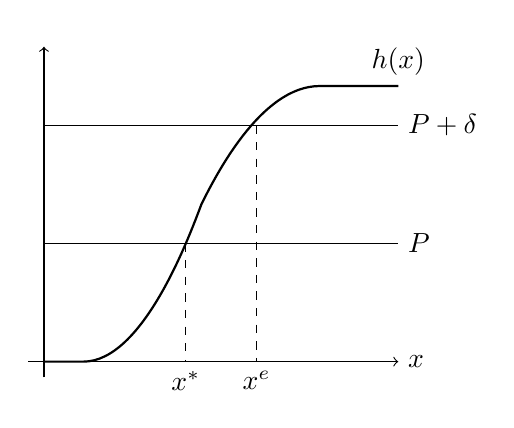
\begin{tikzpicture}[scale=1]
    \draw[->] (-0.2,0) -- (4.5,0) node[right]{$x$}; 
    \draw[->] (0,-0.2) -- (0,4) node[above]{};
    \draw[thick] (0,0) to (0.5,0) parabola (2,2) parabola[bend at end] (3.5,3.5) to (4.5,3.5) node[above]{$h(x)$};
    \draw[thin] (0,1.5) to (4.5,1.5) node[right]{${P}$};
    \draw[dashed, thin] (1.8,1.5) -- (1.8,0) node[below]{$x^*$}; 
    \draw[thin] (0,3) to (4.5,3) node[right]{${P+\delta}$};
    \draw[dashed, thin] (2.7,3) -- (2.7,0) node[below]{$x^e$}; 
\end{tikzpicture}
    \caption{Platform Over-Removal under Strict Liability if $\delta>0$}
    \label{fig:removal}
\end{figure}


\subsection{Imperfect Information and Positive Externality}

The platform is uncertain about whether and to what extent each item is harmful. 
The platform has the prior belief that item $x$ might cause harm $h(x)$ with probability $\lambda(x)\in[0,1]$. Without loss of generality, we assume $\lambda(x)h(x)$ is a weakly increasing function such that the content is ordered by the ascending expected level of harm. We also assume that there is no-harm content ($\lambda(0)=0$) and unambiguously harmful content ($\lambda(1)=1$ and $h(1)=\Bar{h}$).
% And items are heterogeneous in their probability of being harmful. we assume $\lambda(x)$ is a weakly increasing function such that the content is ordered by the ascending likelihood of causing harm.

Given $\hat{x}$, $\int_0^{\hat{x}}\lambda(x)h(x)dx$ is the expected harm given the amount of content $\hat{x}$, and $P\hat{x}$ is the consumer welfare.
The \emph{ex-ante} social welfare function is given by 
\begin{equation}
    \max\{\max_{\hat{x}}P\hat{x}+\delta\hat{x} - \int_0^{\hat{x}}\lambda(x)h(x)dx-F, 0\}.
\end{equation}
Suppose the platform does not shut down, 
the efficient moderation decision $x^e$ is such that
\begin{equation}
    \lambda(x^e)h(x^e)=P+\delta,
\end{equation}
where $P+\delta$ is the marginal social cost of removing the marginal item $x^e$, and $\lambda(x^e)h(x^e)$ is the expected marginal social benefit of removing $x^e$. This is socially efficient if the fixed cost $F$ is not too large.

The analysis can proceed as the last section with the only difference being the expected harm $\lambda(x)h(x)$ instead of the actual harm $h(x)$. Like what we find previously, intermediary immunity is efficient only if the positive externality is sufficiently large. Strict liability lead to over-removal. Negligence based on free speech and safe harbor provision can be efficient. All the liability rules have the same effect except the regime of liability upon notice, which we will elaborate below. 

%% scribe
%% There are going to be two outcomes that are observed here. Outcome one is that this particular item act is harmful. Outcome two, this particular item act is not harmful. 

It is more interesting to consider the environment where the platform can pay an inspection cost $c$ per item to observe a signal of item $x$ indicating whether $x$ is harmful or not. In this case, if the platform chooses to investigate, it can condition its removal decision upon the realization of the signal. The investigation decision will depend upon the cost of investigation and the amount of information the platform gain from it.

%% two alternative ways to solve the problem: 1. mathematical, 2. intuition
Obviously, if the moderation decision remains the same regardless of the realization of the signal, the platform will not incur the cost. 
The signal is useful only if the additional information changes its removal decision. 
Consider content $x\in[0,\hat{x}]$ that will not be removed without investigation. With probability $1-\lambda(x)$ the signal shows no harm and there is no change in the removal decision. With probability $\lambda(x)$ the signal shows harm and this item will be removed. In this case, the marginal value decreases by $P+\delta$ but the marginal harm decreases by $h(x)$, so the net change is $h(x)-P$. This happens with probability $\lambda(x)$, and the expected welfare change is thus $\lambda(x)(h(x)-P-\delta)$.
The social planner prefers the investigation of item $x$ if $\lambda(x)(h(x)-P-\delta)>c$. 
% what we are improving upon it's definitely that you are reducing the harm.

Now consider content $x\in[\hat{x},1]$ that will be removed without investigation. With probability $\lambda(x)$ the signal shows harm and there is no change in the removal decision. With probability $1-\lambda(x)$ the signal shows no harm and this item will not be removed. In either case, the marginal harm $h(x)$ does not show up in the calculation because either the harm has been removed or the investigation finds no harm involved. The benefit of the investigation is to keep the marginal value $P+\delta$ on the platform. The expected welfare change is $(1-\lambda(x))(P+\delta)$. 
The social planner prefers the investigation of item $x$ if $(1-\lambda(x))(P+\delta)>c$. 

Collecting the previous two observations, the social planner wants to pay for the cost only if the welfare improvement exceeds the cost. For $x\ls \hat{x}$, a signal is welfare-improving because it prevents the welfare loss of under-removal. 
%% For $x\ls \hat{x}$, the signal is useful if it reveals the item $x$ is harmful and thus should be removed instead.
Notice that the welfare improvement from under-removal is increasing in $\lambda(x)$.
For $x>\hat{x}$, a signal is welfare-improving because it avoids the welfare loss of over-removal.
Notice that the welfare improvement from over-removal is decreasing in $\lambda(x)$.
% flip the decision

% interval
The next observation is that the platform's investigation decision has to be an interval of items. First notice that there is no value in investigating the no-harm content or the unambiguously harmful content; it is the more ambiguous content in between that provides an incentive for investigation. 
%% And the second observation is that if you want to investigate, it has to be the fact that the lambda has to have a sufficient amount of uncertainty there such that it's beneficial for us to investigate. 
Because of the monotonicity of $\lambda(x)h(x)$, it is suboptimal to pick two disconnected sets and have a gap in between. The platform is always better to join the two sets and leave the less ambiguous items at the ends while keeping the total investigation cost constant. Therefore choosing an interval is a dominant strategy of investigation. 

% now the problem is how to choose the interval
The final step is to determine the optimal choice of the interval. 
An interval is characterized by two parameters: the lower range $\underline{x}$ and the upper range $\overline{x}$. The social planner's problem is as follows:
\begin{equation}
    \max_{\underline{x},\overline{x}} \int_{\underline{x}}^{\overline{x}} [(1-\lambda(x))(P+\delta)-c]dx + \int_0^{\underline{x}} [P+\delta-\lambda(x)h(x)]dx 
\end{equation}
Note that the interval must contain $\hat{x}$ (the moderation decision without investigation). Otherwise, the interval will either contain $x=0$ or $x=1$ leading to a contradiction. 
The lower range $\underline{x}^e$ is determined by the indifference condition of investigating to avoid under-removal (i.e., flip a non-removal decision to a removal decision) such that $\lambda(\underline{x}^e)(h(\underline{x}^e)-P-\delta)=c$. At $\underline{x}^e$, the social planner is just indifferent between paying the cost and the welfare improvement from under-removal. 
The upper range $\overline{x}^e$ is determined by the indifference condition of investigating to avoid over-removal (i.e., flip a removal decision to a non-removal decision) such that $(1-\lambda(\overline{x}^e))(P+\delta)=c$. 

The efficient moderation outcome is to (i) carry $[0,\underline{x}^e)$ and remove $(\overline{x}^e,1]$ without investigation, and (ii) investigate $[\underline{x}^e,\overline{x}^e]$ and remove if it is found harmful and carry otherwise.  
The efficient investigation decision varies with the cost $c$. If $c=0$ such that investigation is costless, the optimal interval is $[0,1]$ that covers the entire content spectrum. As $c$ grows, the interval shrinks until it does not make sense to investigate at all (i.e., $c\ls\frac{P(h(x^e)-P)}{h(x^e)}$, a sufficient condition is $c\ls\frac{P\delta}{P+\delta}$). When $c$ is sufficiently large, we are back in an environment as if no investigation technology is available.


\textbf{Intermediary immunity}.
Because the platform faces no liability for any harm, it does not have any incentive to investigate the harm. It will not pay for the signal as it will carry all the content regardless of the harm. Compared with the social optimum, immunity leads the platform to under-investigate and under-remove. 

\textbf{Strict liability}.
Under strict liability, the platform's investigation problem becomes 
\begin{equation}
    \max_{\underline{x},\overline{x}} \int_{\underline{x}}^{\overline{x}} [(1-\lambda(x))P-c]dx + \int_0^{\underline{x}} [P-\lambda(x)h(x)]dx 
\end{equation}
Note that the platform does not take the positive externality into account, and in calculating the investigation trade-off it only cares about the change in the marginal revenue $P$ (as opposed to $P+\delta$). 
% the idea that you've seen the removal part, but now in the investigation world, you still want to have the same set that the marginal benefit of your investigation covers your cost of the investigation.
% All the stars are for the platform, all the e are for the efficiency. that's why you see in this graph, c is showing up for every single line.
Figure 6 extends figure 5 and compares the socially optimal investigation with the platform's investigation under strict liability. The platform's investigation decision is $[\underline{x}^*,\overline{x}^*]$ where the lower range and the upper range are identified by the intersection of $\lambda(x)$ and the two lines of marginal private cost $\frac{c}{h-P}$ and $1-\frac{c}{P}$. 
In contrast, the lower range and the upper range required by efficiency are located at the intersection of $\lambda(x)$ and the two lines of marginal social cost $\frac{c}{h-(P+\delta)}$ and $1-\frac{c}{P+\delta}$.  
We observe that the platform's interval is always lower than the efficient interval. The decision to investigate $[\underline{x}^e,\overline{x}^*]$ is efficient, but the deicision to investigate $[\underline{x}^*,\underline{x}^e]$ as opposed to $[\overline{x}^*,\overline{x}^e]$ is inefficient. In this sense, we say the platform is biased in investigation under strict liability. Strict liability leads the platform to investigate the \emph{wrong} types. This happens because the platform cannot internalize the positive externality of the content. The consequence of under-investigation is over-removal. The platform is doing uninformed removal of the upper tail $[\overline{x}^*,\overline{x}^e]$, and is having excessive scrutiny over the lower tail $[\underline{x}^*,\underline{x}^e]$. As a result, the platform is carrying too little content.

% platform make blunter decisions to take down too much content at the lower end of the range or to leave up too much content at the upper end of the range. 

\begin{figure}[h]
    \centering
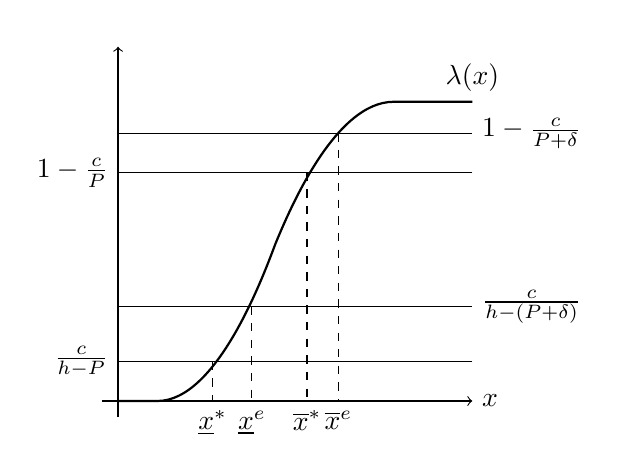
\begin{tikzpicture}[scale=1]
    \draw[->] (-0.2,0) -- (4.5,0) node[right]{$x$}; 
    \draw[->] (0,-0.2) -- (0,4.5) node[above]{};
    \draw[thick] (0,0) to (0.5,0) parabola (2,2) parabola[bend at end] (3.5,3.8) to (4.5,3.8) node[above]{$\lambda(x)$};
    %% next four \draw are efficiency
    \draw[thin] (0,1.2) to (4.5,1.2) node[right]{$\frac{c}{h-(P+\delta)}$};
    \draw[thin] (0,3.4) to (4.5,3.4) node[right]{$1-\frac{c}{P+\delta}$};
    \draw[dashed, thin] (1.7,1.2) -- (1.7,0) node[below]{$\underline{x}^e$};
    \draw[dashed, thin] (2.8,3.4) -- (2.8,0) node[below]{$\overline{x}^e$};
    %% next four \draw are profit
    \draw[thin] (4.5,0.5) to (0,0.5) node[left]{$\frac{c}{h-P}$}; 
    \draw[thin] (4.5,2.9) to (0,2.9) node[left]{$1-\frac{c}{P}$};
    \draw[dashed, thin] (1.2,0.5) -- (1.2,0) node[below]{$\underline{x}^{\ast}$};
    \draw[dashed, thin] (2.4,2.9) -- (2.4,0) node[below]{$\overline{x}^{\ast}$};   
\end{tikzpicture}
    \caption{Biased Investigation of the Platform under Strict Liability if $\delta>0$}
    \label{fig:investigation}
\end{figure}


\textbf{Free speech law}.
Notice that $\underline{x}^e$ has two roles in the efficient solution: it is the lower bound for investigation, \emph{and} the upper bound for removal without investigation. It is a natural threshold for the reasonable person standard in this environment. The negligence rule is thus
\begin{equation}
d(x)=
\lt\{\begin{array}{ll}
    h(x) & \mbox{if $x$ is not removed and $x\in[\underline{x}^e,1]$}, \\ % part of x
    0 & \mbox{otherwise}.
\end{array}\rt.
\end{equation}
The free speech region is $[0,\underline{x}^e]$ where carrying any content leads to no liability and the negligence region is $[\underline{x}^e,1]$ where carrying any content leads to strict liability. 
Platform's problem under this rule is 
\begin{equation}
    \max_{\underline{x},\overline{x}} \int_{\underline{x}}^{\overline{x}} [(1-\lambda(x))P-c]dx + \int_0^{\underline{x}} [P-\lambda(x)h(x)I(x\in[\underline{x}^e,1])]dx 
\end{equation}
This takes into account the fact that if the investigation interval overlaps with the negligence region, the platform will remove the content to avoid liability. First, notice that $\underline{x}$ is at least $\underline{x}^e$ otherwise it contradicts profit maximization. Next notice that the marginal revenue of moving just above $\underline{x}^e$ is negative as $\lambda(\underline{x}^e)[P-h(\underline{x}^e)]+c=-\lambda(\underline{x}^e)\delta<0$. Thus $\underline{x}$ is at most $\underline{x}^e$ and it follows that $\underline{x}^*=\underline{x}^e$. The lower range choice is efficient under the free speech law. The upper range choice, however, will not be efficient. The platform will choose $\overline{x}^*$ such that $(1-\lambda(\overline{x}^*))P=c$. As $[\underline{x}^*,\overline{x}^*]\subset[\underline{x}^e,\overline{x}^e]$, The platform shirks its effort on investigation, and the inefficiency problem is under-investigation.  


\textbf{Safe harbor provision}.
Defining a standard for total harm is not obvious here. There are two choices we can consider: \emph{ex-ante} total harm and \emph{ex-post} total harm.
Setting the standard on \emph{ex-post} total harm is hard to monitor. Suppose the rule is conditional on the investigation such that if the platform finds the content harmful, failure to remove it will result in liability. It actually provides the platform with disincentive to find out about the content in the first place.  

% revisit the efficient objective
A safe harbor provision that caps the \emph{ex-ante} total harm can be formulated as follows:
\begin{equation}
d(x)=
\lt\{\begin{array}{ll}
    h(x) & \mbox{if $\int_0^{\underline{x}}\lambda(x)h(x)dx>s_h=\int_0^{\underline{x}^e}\lambda(x)h(x)dx$}, \\
    0 & \mbox{otherwise}.
\end{array}\rt.
\end{equation}
Suppose the platform chooses $\underline{x}>\underline{x}^e$ such that it loses the safe harbor status, the penalty in liability would be $\int_0^{\underline{x}}\lambda(x)h(x)dx$ whereas the gain in revenue would be $\int_{\underline{x}^e}^{\underline{x}}[\lambda(x)P+c]$. The deviation is not profitable.
The optimal choice $\underline{x}^*$ is equal to $\underline{x}^e$ such that the platform maximizes the profits without losing its safe harbor status. 
\footnote{It is sub-optimal to carry items of higher types while keeping the total harm constant, which results in less content and thus less revenue.}

For $x>\underline{x}$, the platform wants to carry as much content as possible but fears going beyond the safe harbor limit. The platform has an incentive to investigate to keep the safe harbor status. It will do so until the marginal expected revenue $(1-\lambda(x))P$ can no longer justify the investigation cost $c$. The upper range $\overline{x}^*$ is such that $(1-\lambda(\overline{x}^*))=c$. 
Since $\overline{x}^*<\overline{x}^e$, platform under-investigate.
Setting the standard on total harm alone does not provide sufficient incentive for investigation.

However, a safe harbor provision may not only be conditioned on the total harm, but can also be conditioned on other observables. And in fact, a safe harbor provision directly regulating the investigation effort can lead to the efficient moderation outcome. A safe harbor provision, that both caps the total harm and requires a floor on total investigation cost, is characterized by a pair of standards $(s_h,s_c)$ such that:
\begin{equation}
d(x)=
\lt\{\begin{array}{ll}
    0 & \mbox{if $\int_0^{\underline{x}}\lambda(x)h(x)dx\ls s_h$ and $c[\overline{x}-\underline{x}]\gs s_c$}, \\
    h(x) & \mbox{otherwise}.
\end{array}\rt.
\end{equation}
We know from our previous discussion that the platform prefers to keep the safe harbor status. Because of the requirement of minimal effort, the platform would investigate at least up to the efficient upper bound such that $\overline{x}^*\gs\overline{x}^e$. Will the platform investigate more than necessary ? It will not. As the profit change at $\overline{x}^e$ is negative, i.e., $(1-\lambda(\overline{x}^e))P-c=-(1-\lambda(\overline{x}^e))\delta<0$.  

Therefore, we can formulate the platform's problem as profit maximization subject to two policy constraints:
\begin{eqnarray}
\max_{\underline{x},\overline{x}} &&
\hspace{-1em} P\underline{x}+\int_{\underline{x}}^{\overline{x}} [(1-\lambda(x))P-c]dx \nn\\
\mbox{s.t.} &&\hspace{-1em} \int_0^{\underline{x}}\lambda(x)h(x)dx\ls s_h, \nn\\
&&\hspace{-1em} c[\overline{x}-\underline{x}]\gs s_c.
\end{eqnarray}
If the pair of threshold is chosen properly such that $s_h=\int_0^{\underline{x}^e}\lambda(x)h(x)dx$ and $s_c=c[\overline{x}^e-\underline{x}^e]$. 
The two constraints are binding such that $\underline{x}^*=\underline{x}^e$ and $\overline{x}^*=\overline{x}^e$.
Safe harbor provision leads to the efficient moderation outcome.


\textbf{Liability Upon Notice}.
%% platform's strategy is not an interval
%% this should be a PBE; users may not be truthful?
The notice serves the same function as a signal that tells the platform whether the item in question is harmful or not. In that sense, liability upon notice shifts the cost of investigation to the harmed parties.
We will start with the assumption that the platform does not investigate in addition to the notices. The platform's decision would be a threshold denoted by $\underline{x}^*$. Equivalently for comparison, we can also think of the platform choosing an interval $[\underline{x}^*,1]$. We will then relax this assumption and allow the platform to investigate. We will see that the platform has no incentive to do extra investigations. 

Users, being completely informed, will send a notice if and only if $h(x)\gs c$. 
For items $x\in[0,h^{-1}(c))$, the platform is not liable for any harm, thus $\underline{x}^*$ is at least $h^{-1}(c)$. For items $x\in[h^{-1}(c),1]$, there is a probability $1-\lambda(x)$ that no notice is received and if that happens, the platform will carry the content. There is a probability $\lambda(x)$ that the platform receives a notice, in which case it will remove $x$ if $P<h(x)$. If $P\ls c$, every notice leads to a takedown. If instead $P>c$, some notices do not lead to a takedown, and $h(\underline{x}^*)=P$. Thus in this sequential move game, the platform will set $\underline{x}^*$ such that $h(\underline{x}^*)=\max\{P,c\}$. Suppose we allow the platform to investigate, it is easy to show that it is not profitable to investigate any item $x\in[0,h^{-1}(c))$.

The welfare implied by the platform's decision and the users' notice choice can be evaluated from the social planner's \emph{ex-ante} perspective:
\begin{equation}
(P+\delta)\underline{x}^*+\int_{\underline{x}^*}^1 (1-\lambda(x))(P+\delta)dx-\int_{h^{-1}(c)}^{\max\{\underline{x}^*,h^{-1}(c)\}}\lambda(x)h(x)dx-\int_{h^{-1}(c)}^{1}\lambda(x)cdx
\end{equation}
Compared with the efficiency solution, notice that $h(\underline{x}^*)=\max\{P,c\}<P+\delta+\frac{c}{\lambda(\underline{x}^e)}=h(\underline{x}^e)$. It follows that $\underline{x}^*<\underline{x}^e$ and $[\underline{x}^e,\overline{x}^e]\subset[\underline{x}^*,1]$. 
Liability upon notice is not efficient even though it saves the platform's cost of acquiring information. 
The inefficiency comes from the fact that the notice procedure is over-used, and too many notices lead the platform to carry too little content.





%% The platform receives a revenue of $R \ge 0$ for each item it carries, good or bad. It can tell the difference between the two types at a cost of $C \ge 0$ per item. If it decides to remove an item of content, it gives up the revenue associated with that item.

% Putting this all together, the case for intermediary immunity is justified when $C > C^*$ and $\beta < G/(B+G)$ (one paragraph explains C*, one explain C>C*, one explain second inequality) Effective filtering is cost-prohibitive, so that imposing liability will lead the platform to overfilter (from society's point of view) by shutting down. But since society prefers to have the platform to not having it (because the good content still outweighs the bad), it is better off with underfiltering than overfiltering.


%must carry or must remove rule
%Must remove rule
% Q. loss of safe harbor means all the content is liable for $d$, or only part of the content liable for $d$.

%(i) If all the platform can do is content removal and no positive externality, strict liability leads to efficiency.
%(ii) content removal + positive externality, strict liability leads to over-removal and immunity might be justified if the externality is sufficiently large (though that means keeping all the content).
%(iii) If platform can first choose whether to investigate and then decide on removal, with no positive externality, strict liability again leads to efficiency !
%(iv) investigate + removal + positive externality, strict liability leads to under-investigation and over-removal.  
%(v) imperfect signal does not change (iii) and (iv). 

% (iii)For complete info+no externality, (b)(c)(d)(e) can all lead to efficient outcome.
% (iv)For complete info+positive externality, (a) can be efficient under some condition. (b)(e) lead to over-removal. (c)(d) lead to efficient outcome.
% v) For incomplete info+positive externality, (a)(b)(c)(e) are all sub-optimal. There might be some version of (d) that leads to efficient outcome (I'm still figuring that out).

In conclusion, many liability rules fail in this rich environment where content has positive externality, the platform has imperfect information regarding the harm, information can be transmitted either through investigation or through notices. Immunity, strict liability, free speech, and liability upon notice are all inefficient. The only efficient rule is a safe harbor provision based on total harm and reasonable effort.

\begin{proposition}
Given imperfect information and positive externality, a safe harbor provision, which both caps the total harm and requires a minimal effort on investigation, leads to the efficient moderation outcome. 
\end{proposition}